\documentclass[12pt,letterpaper]{exam}
\usepackage[lmargin=1in,rmargin=1in,tmargin=1in,bmargin=1in]{geometry}
\usepackage{../style/exams}

% -------------------
% Course & Exam Information
% -------------------
\newcommand{\course}{MATH 142: Exam 1}
\newcommand{\term}{Spring ---\textsubscript{\textsubscript{2}} 2026}
\newcommand{\examdate}{02/12/2026}
\newcommand{\timelimit}{75 Minutes}

\setbool{hideans}{false} % Student: True; Instructor: False

\newcommand{\boxseven}[4]{%
	\draw[thick] (0,0) -- (4,0) -- (4,4) -- (0,4) -- (0,0);
	\draw[thick] (0,2) -- (4,2);
	\draw[thick] (2,0) -- (2,4);
	% '7'
	\draw[line width=0.03cm] (1.7,2.2) -- (2.3,2.2) -- (1.7,1.6);
	% Entries
	\node at (1,3) {$#1$};	% u
	\node at (3,1) {$#2$};	% dv
	\node at (1,1) {$#3$};	% du
	\node at (3,3) {$#4$};	% v
}


\usetikzlibrary{calc}
\usepackage{booktabs}
\tikzset{Arrow Style/.style={text=black, font=\boldmath}}
\newcommand{\tikzmark}[1]{%
    \tikz[overlay, remember picture, baseline] \node (#1) {};%
}
\newcommand*{\XShift}{0.5em}
\newcommand*{\YShift}{0.5ex}
\NewDocumentCommand{\DrawArrow}{s O{} m m m}{%
    \begin{tikzpicture}[overlay,remember picture]
        \draw[->, thick, Arrow Style, #2] 
                ($(#3.west)+(\XShift,\YShift)$) -- 
                ($(#4.east)+(-\XShift,\YShift)$)
        node [midway,above] {#5};
    \end{tikzpicture}%
}

\usepackage{cancel}

% -------------------
% Content
% -------------------
\begin{document}

\examtitle
\instructions{Write your name on the appropriate line on the exam cover sheet. This exam contains \numpages\ pages (including this cover page) and \numquestions\ questions. Check that you have every page of the exam. Answer the questions in the spaces provided on the question sheets. Be sure to answer every part of each question and show all your work. If you run out of room for an answer, continue on the back of the page --- being sure to indicate the problem number.
} 
\scores
\bottomline
\newpage


% -------------------
% Questions
% -------------------
\begin{questions}

% Question 1
\newpage
\question[10] Showing all your work and completely simplifying your result, compute the following:
	\[
	\int_0^\pi x \sec^2 \left( \dfrac{x}{4} \right) \;dx
	\] \par\vspace{0.3cm}

\vsol{\itshape We can integrate-by-parts. Using LIATE, we choose $u= x$ (`A' for algebraic) and so $dv= \sec^2 \left( \tfrac{x}{4} \right)$. We then have\dots
	\[
	\begin{tikzpicture}
	\boxseven{x}{\sec^2 \left( \tfrac{x}{4} \right)}{1}{4\tan \left( \tfrac{x}{4} \right)}
	\end{tikzpicture}
	\] \pspace
Therefore, we have\dots
	\[
	\begin{aligned}
	\int_0^\pi x \sec^2 \left( \dfrac{x}{4} \right) \;dx&= 4x \tan \left( \tfrac{x}{4} \right) \bigg|_0^\pi - \int_0^\pi 4\tan \left( \tfrac{x}{4} \right) \;dx \\[0.3cm]
	&= 4x \tan \left( \tfrac{x}{4} \right) \bigg|_0^\pi - 16 \ln \left| \sec \left( \tfrac{x}{4} \right) \right| \bigg|_0^\pi \\[0.3cm]
	&= 4x \tan \left( \tfrac{x}{4} \right) \bigg|_0^\pi - 16 \ln \left| \sec \left( \tfrac{x}{4} \right) \right| \bigg|_0^\pi \\[0.3cm]
	&= 4 \left[ \pi \tan\left( \frac{\pi}{4} \right) - 0 \tan(0) \right] - 16 \left[ \ln \left| \sec \left( \tfrac{\pi}{4} \right) \right| - \ln \left| \sec \left( 0 \right) \right| \right] \\[0.3cm]
	&= 4 \left[ \pi \cdot 1 - 0 \right] - 16 \left[ \ln| \sqrt{2} | - \ln|1| \right] \\[0.3cm]
	&= 4 \pi - 16 \left[ \ln| \sqrt{2} | - 0 \right] \\[0.3cm]
	&= \boxed{4 \pi - 16 \ln(\sqrt{2})} \\[0.3cm]
	&= 4 \pi - 16 \cdot \tfrac{1}{2} \ln(2) \\[0.3cm]
	&= 4\pi - 8 \ln 2 \\[0.3cm]
	&= 4(\pi - 2 \ln 2)
	\end{aligned}
	\]
}



% Question 2
\newpage
\question[10] Determine whether the integral below converges or diverges. If it converges, find its value. If it diverges, explain why. Be sure to show all your work and full simplify your answer.
	\[
	\int_{-\infty}^{\sqrt{3}} \dfrac{dx}{1 + x^2} 
	\] \par\vspace{0.3cm}

\vsol{\itshape Because of the `$-\infty$' in the limits of integration, the integral is improper. We first find an antiderivative. We know that\dots
	\[
	\int \dfrac{dx}{1 + x^2}= \arctan x + C
	\]
Therefore, we have\dots
	\[
	\begin{aligned}
	\int_{-\infty}^{\sqrt{3}} \dfrac{dx}{1 + x^2}&:= \lim_{b \to -\infty} \int_{b}^{\sqrt{3}} \dfrac{dx}{1 + x^2} \\[0.3cm]
	&= \lim_{b \to -\infty} \arctan x \bigg|_b^{\sqrt{3}} \\[0.3cm]
	&= \arctan \left( \sqrt{3} \right) - \lim_{b \to -\infty} \arctan b \\[0.3cm]
	&= \dfrac{\pi}{3} - \dfrac{-\pi}{2} \\[0.3cm]
	&= \dfrac{2\pi}{6} + \dfrac{3\pi}{6} \\[0.3cm]
	&= \boxed{\dfrac{5\pi}{3}}
	\end{aligned}
	\]
Therefore, the integral converges to $\frac{5\pi}{3}$.}



% Question 3
\newpage
\question[10] Showing all your work and completely simplifying your result, compute the following:
	\[
	\int \dfrac{-5x^2 + 5x + 5}{(2x + 1)(x^2 + 3)} \;dx
	\] \par\vspace{0.3cm}

\vsol{\itshape We use partial fractions. The degree of the numerator is two while the degree of the denominator is $1 + 2= 3$. So, we need not perform polynomial long division. The denominator is already completely factored. The partial fraction decomposition then takes the form\dots
	\[
	\begin{aligned}
	\dfrac{-5x^2 + 5x + 5}{(2x + 1)(x^2 + 3)}&= \dfrac{A}{2x + 1} + \dfrac{Bx + C}{x^2 + 3} \\[0.3cm]
	&= \dfrac{A(x^2 + 3) + (Bx + C)(2x + 1)}{(2x + 1)(x^2 + 3)}
	\end{aligned}
	\]
Because the denominators are equal, the numerators must be equal. Therefore, we have\dots
	\[
	\begin{gathered}
	-5x^2 + 5x + 5= A(x^2 + 3) + (Bx + C)(2x + 1) \\
	-5x^2 + 5x + 5= (Ax^2 + 3A) + (2Bx^2 + Bx + 2Cx + C) \\
	-5x^2 + 5x + 5= (A + 2B)x^2 + (B + 2C)x + (3A + C)
	\end{gathered}
	\]
Therefore, we have\dots \par
	\[
	\begin{aligned}
	x^2&\colon & -5&= A + 2B \\
	x&\colon & 5&= B + 2C \\
	1&\colon & 5&= 3A + C
	\end{aligned}
	\]
Subtracting twice the second equation from the first, we have $-15= A - 4C$. Adding this to four times the third equation, we find $5= 13A$, which implies that $A= \tfrac{5}{13}$. [Alternatively, by Heaviside's, we know that $A= \tfrac{-5(-1/2)^2 + 5(-1/2) + 5}{(-1/2)^2 + 3}= \tfrac{-5/4 - 5/2 + 5}{1/4 + 3}= \tfrac{5/4}{13/4}= \tfrac{5}{13}$.] But then $-5= \tfrac{5}{13} + 2B$, i.e. $-65= 5 + 26B$, so that $B= -\tfrac{35}{13}$. Finally, we have $5= 3(\tfrac{5}{13}) + C$, i.e. $65= 15 + 13C$, which implies $C= \frac{50}{13}$. Therefore, we have\dots
	\[
	\int \dfrac{-5x^2 + 5x + 5}{(2x + 1)(x^2 + 3)} \;dx= \int \left( \dfrac{\tfrac{5}{13}}{2x + 1} + \dfrac{-\tfrac{35}{13}\,x + \tfrac{50}{13}}{x^2 + 3} \right) \;dx= \int \left( \dfrac{\tfrac{5}{13}}{2x + 1} + \dfrac{-\tfrac{35}{13}\,x}{x^2 + 3} + \dfrac{\tfrac{50}{13}}{x^2 + 3} \right) \;dx
	\]
Using the fact that the antiderivative of $\frac{ax}{x^2 + b}= \frac{a}{2} \ln|x^2 + b|$ (this can be found using the $u$-substitution $u= x^2 + b$), the antiderivative of $\frac{1}{x^2 + a^2}= \frac{1}{a} \arctan\left( \tfrac{x}{a} \right) + C$, and the fact $x^2 + 3= x^2 + (\sqrt{3})^2$, we have\dots
	\[
	\int \left( \dfrac{\tfrac{5}{13}}{2x + 1} + \dfrac{-\tfrac{35}{13}\,x}{x^2 + 3} + \dfrac{\tfrac{50}{13}}{x^2 + 3} \right) \;dx= \frac{5}{26} \ln|2x + 1| - \tfrac{35}{26} \ln|x^2 + 3| + \dfrac{50}{13\sqrt{3}} \, \arctan\left( \dfrac{x}{\sqrt{3}} \right) + K
	\]
Therefore, we know\dots
	\[
	\boxed{\int \dfrac{-3x^2 + 4x + 8}{(2x + 1)(x^2 + 5)} \;dx= \frac{5}{26} \ln|2x + 1| - \tfrac{35}{26} \ln|x^2 + 3| + \dfrac{50}{13\sqrt{3}} \, \arctan\left( \dfrac{x}{\sqrt{3}} \right) + K}
	\]
}
%	\[
%	\int \dfrac{-5x^2 + x + 5}{(2x + 1)(x^2 + 3)} \;dx
%	\] \par\vspace{0.3cm}
%
%\vsol{\itshape We use partial fractions. The degree of the numerator is two while the degree of the denominator is $1 + 2= 3$. So, we need not perform polynomial long division. The denominator is already completely factored. The partial fraction decomposition then takes the form\dots
%	\[
%	\begin{aligned}
%	\dfrac{-5x^2 + x + 5}{(2x + 1)(x^2 + 3)}&= \dfrac{A}{2x + 1} + \dfrac{Bx + C}{x^2 + 3} \\
%	&= \dfrac{A(x^2 + 3) + (Bx + C)(2x + 1)}{(2x + 1)(x^2 + 3)}
%	\end{aligned}
%	\]
%Because the denominators are equal, the numerators must be equal. Therefore, we have\dots
%	\[
%	\begin{gathered}
%	-5x^2 + x + 5= A(x^2 + 3) + (Bx + C)(2x + 1) \\
%	-5x^2 + x + 5= (Ax^2 + 3A) + (2Bx^2 + Bx + 2Cx + C) \\
%	-5x^2 + x + 5= (A + 2B)x^2 + (B + 2C)x + (3A + C)
%	\end{gathered}
%	\]
%Therefore, we have\dots \par
%	\[
%	\begin{aligned}
%	x^2&\colon & -5&= A + 2B \\
%	x&\colon & 1&= B + 2C \\
%	1&\colon & 5&= 3A + C
%	\end{aligned}
%	\]
%Subtracting twice the second equation from the first, we have $-7= A - 4C$. Adding this to four times the third equation, we find $13= 13A$, which implies that $A= 1$. [Alternatively, by Heaviside's, we know that $A= \tfrac{-5(-1/2)^2 + (-1/2) + 5}{(-1/2)^2 + 3}= \tfrac{-5/4 - 1/2 + 5}{1/4 + 3}= \tfrac{13/4}{13/4}= 1$.] But then $-5= 1 + 2B$, so that $B= -3$. Finally, we have $5= 3(1) + C$, which implies $C= 2$. Therefore, we have\dots
%	\[
%	\int \dfrac{-5x^2 + x + 5}{(2x + 1)(x^2 + 3)} \;dx= \int \left( \dfrac{1}{2x + 1} + \dfrac{-3x + 2}{x^2 + 3} \right) \;dx= \int \left( \dfrac{1}{2x + 1} + \dfrac{-3x}{x^2 + 3} + \dfrac{2}{x^2 + 3} \right) \;dx
%	\]
%Using the fact that the antiderivative of $\frac{ax}{x^2 + b}= \frac{a}{2} \ln|x^2 + b|$ (this can be found using the $u$-substitution $u= x^2 + b$), the antiderivative of $\frac{1}{x^2 + a^2}= \frac{1}{a} \arctan\left( \tfrac{x}{a} \right) + C$, and the fact $x^2 + 3= x^2 + (\sqrt{3})^2$, we have\dots
%	\[
%	\int \left( \dfrac{1}{2x + 1} + \dfrac{-3x}{x^2 + 3} + \dfrac{2}{x^2 + 3} \right) \;dx= \tfrac{1}{2} \ln|2x + 1| - \tfrac{3}{2} \ln|x^2 + 3| + \dfrac{2}{\sqrt{3}} \, \arctan\left( \dfrac{x}{\sqrt{3}} \right) + K
%	\]
%Therefore, we know\dots
%	\[
%	\boxed{\int \dfrac{-3x^2 + 4x + 8}{(2x + 1)(x^2 + 5)} \;dx= \tfrac{1}{2} \ln|2x + 1| - \tfrac{3}{2} \ln|x^2 + 3| + \dfrac{2}{\sqrt{3}} \, \arctan\left( \dfrac{x}{\sqrt{3}} \right) + K}
%	\]
%}



% Question 4
\newpage
\question[10] Showing all your work and completely simplifying your result, compute the following:
	\[
	\int (3x + 1)^3\, e^{-x} \;dx
	\] \par\vspace{0.3cm}

\vsol{\itshape Because this is of the form polynomial function times exponential function, we use integration-by-parts---specifically, tabular integration. Using LIATE, we continually choose $u$ to be the polynomial and $dv$ to be the exponential part. We then have\dots
	\[
	\begin{array}{r @{\hspace*{1.3cm}} c} \toprule
	u & dv \\ \cmidrule(lr){1-2}
	(3x + 1)^3 \tikzmark{Left 1} & \tikzmark{Right 1} e^{-x} \\[0.3cm]
	3(3x + 1)^2 \cdot 3= 9(3x + 1)^2 \tikzmark{Left 2} & \tikzmark{Right 2} -e^{-x} \\[0.3cm]
	18(3x + 1)^1 \cdot 3= 54(3x + 1) \tikzmark{Left 3} & \tikzmark{Right 3} e^{-x} \\[0.3cm]
	54 \cdot 3= 162 \tikzmark{Left 4} & \tikzmark{Right 4} -e^{-x} \\[0.3cm]
	0 \tikzmark{Left 5} & \tikzmark{Right 5} e^{-x}
	
	\DrawArrow{Left 1}{Right 2}{+}
	\DrawArrow{Left 2}{Right 3}{--}
	\DrawArrow{Left 3}{Right 4}{+}
	\DrawArrow{Left 4}{Right 5}{--}
	\end{array}
	\]
Therefore, we have\dots
	\[
	\begin{aligned}
	\int (3x + 1)^3\, e^{-x} \;dx&= \boxed{-(3x + 1)^3 e^{-x} - 9(3x + 1)^2 e^{-x} - 54(3x + 1)e^{-x} - 162 e^{-x} + C} \\[0.3cm]
	&= -e^{-x} \left( (3x + 1)^3 + 9(3x + 1)^2 + 54(3x + 1) + 162 \right) + C \\[0.3cm]
	&= -e^{-x} \left( 27x^3 + 108x^2 + 225x + 226 \right) + C
	\end{aligned}
	\]
}



% Question 5
\newpage
\question[10] Showing all your work and completely simplifying your result, compute the following:
	\[
	\int \sec^9(\theta) \tan^3(\theta) \;d\theta
	\] \par\vspace{0.3cm}

\vsol{\itshape This is a trigonometric integral. We choose $u= \sec \theta$. So then $du= \sec \theta \tan \theta \;d\theta$. Using the fact that $\sin^2 \theta + \cos^2 \theta= 1$, we know that $\tan^2 \theta + 1= \sec^2 \theta$, i.e. $\tan^2 \theta= \sec^2 \theta - 1$. But then\dots
	\[
	\begin{aligned}
	\int \sec^9(\theta) \tan^3(\theta) \;d\theta&= \int \sec^8 \theta \tan^2 \theta \cdot \sec \theta \tan \theta \;d\theta \\[0.3cm]
	&= \int \sec^8(\theta) (\sec^2 \theta - 1) \cdot \sec \theta \tan \theta \;d\theta \\[0.3cm]
	&= \int u^8 (u^2 - 1) \;du \\[0.3cm]
	&= \int \left( u^{10} - u^8 \right) \;du \\[0.3cm]
	&= \dfrac{u^{11}}{11} - \dfrac{u^9}{9} + C \\[0.3cm]
	&= \boxed{\dfrac{\sec^{11} \theta}{11} - \dfrac{\sec^9 \theta}{9} + C} \\[0.3cm]
	&= \dfrac{\sec^9 \theta}{99} \left( 9 \sec^2 \theta - 11 \right) + C
	\end{aligned}
	\]
}



% Question 6
\newpage
\question[10] Showing all your work and completely simplifying your result, compute the following:
	\[
	\int x \sqrt{x - 3} \;dx
	\] \par\vspace{0.3cm}

\vsol{\itshape Using $u$-substitution, we choose $u= x - 3$, so that $du= dx$. Because $u= x - 3$, we have $x= u + 3$. But then\dots
	\[
	\begin{aligned}
	\int x \sqrt{x - 3} \;dx&= \int (u + 3) \sqrt{u} \;du \\[0.1cm]
	&= \int \left( u^{3/2} + 3 u^{1/2} \right) \;du \\[0.1cm]
	&= \dfrac{2u^{5/2}}{5} + \dfrac{2(3)u^{3/2}}{3} + C \\[0.1cm]
	&= \boxed{\dfrac{2(x - 3)^{5/2}}{5} + 2(x - 3)^{3/2} + C} \\[0.1cm]
	&= \dfrac{2}{5}\,(x - 3)^{3/2} \big( (x - 3) + 5 \big) + C \\[0.1cm]
	&= \dfrac{2}{5}\, (x - 3)^{3/2} \big(x + 2 \big) + C
	\end{aligned}
	\]
Alternatively, we can use integration-by-parts. Choosing $u= x$ and $dv= \sqrt{x - 5}$, we have\dots
	{\footnotesize
	\[
	\begin{tikzpicture}
	\boxseven{x}{\sqrt{x - 3}}{1}{\tfrac{2}{3}\,(x - 3)^{3/2}}
	\end{tikzpicture}
	\] 
	}
We then have\dots
	\[
	\begin{aligned}
	\int x \sqrt{x - 3} \;dx&= \dfrac{2}{3}\, x(x - 3)^{3/2} - \int \dfrac{2}{3}\,(x - 3)^{3/2} \;dx \\[0.1cm]
	&= \boxed{\dfrac{2}{3}\, x(x - 3)^{3/2} - \dfrac{4}{15}\,(x - 3)^{5/2} + C} \\[0.1cm]
	&= \dfrac{2}{15} (x - 3)^{3/2} \big(5x - 2(x - 3) \big) + C \\[0.1cm]
	&= \dfrac{2}{15} (x - 3)^{3/2} \big(3x + 6 \big) + C \\[0.1cm]
	&= \dfrac{2}{15} (x - 3)^{3/2} \cdot 3 \big(x + 2 \big) + C \\[0.1cm]
	&= \dfrac{2}{5} (x - 3)^{3/2} \big(x + 2 \big) + C
	\end{aligned}
	\]
}

\vsol{
\newpage
{
\thispagestyle{empty}
\itshape Alternatively, we can use trig. substitution. We know from the Pythagorean Theorem that $a^2 + b^2= c^2$, which implies that $a^2= c^2 - b^2$. Taking $c^2= x$, i.e. $c= \sqrt{x}$, and $b^2= 3$, i.e. $b= \sqrt{3}$, we have $a^2= c^2 - b^2= x - 3$. This also shows that $a= \sqrt{x - 3}$. There are two possible right triangles corresponding to these sides we could draw:
	\[
	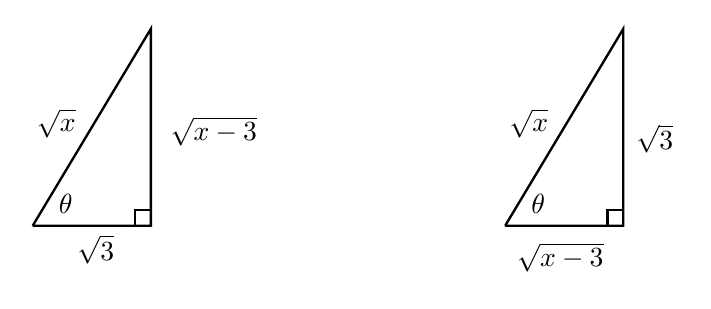
\begin{tikzpicture}
	\draw[line width=0.03cm] (0,0) -- (1.5,0) -- (1.5,2.5) -- (0,0);
	\draw[line width=0.03cm] (1.3,0) -- (1.3,0.2) -- (1.5,0.2);
	\node at (0.8,-0.3) {$\sqrt{3}$};
	\node at (2.3,1.2) {$\sqrt{x - 3}$};
	\node at (0.3,1.3) {$\sqrt{x}$};
	\node at (0.42,0.28) {$\theta$};
	
	\tikzset{shift={(6,0)}};

	\draw[line width=0.03cm] (0,0) -- (1.5,0) -- (1.5,2.5) -- (0,0);
	\draw[line width=0.03cm] (1.3,0) -- (1.3,0.2) -- (1.5,0.2);
	\node at (1.9,1.1) {$\sqrt{3}$};
	\node at (0.7,-0.4) {$\sqrt{x - 3}$};
	\node at (0.3,1.3) {$\sqrt{x}$};
	\node at (0.42,0.28) {$\theta$};
	\end{tikzpicture}
	\]
Using the right triangle on the left, we have $\cos \theta= \frac{\sqrt{3}}{\sqrt{x}}$, so that $\sqrt{x}= \frac{\sqrt{3}}{\cos \theta}= \sqrt{3} \sec \theta$. So, $x= (\sqrt{x})^2= (\sqrt{3} \sec \theta)^2= 3 \sec^2 \theta$. But then $dx= 6 \sec \theta \cdot \sec \theta \tan \theta \;d\theta= 6 \sec^2 \theta \tan \theta \;d\theta$. Observe that $\tan \theta= \frac{\sqrt{x - 3}}{\sqrt{3}}$, so that $\sqrt{x - 3}= \sqrt{3} \tan \theta$. But then\dots
	\[
	\int x \sqrt{x - 3} \;dx= \int 3 \sec^2 \theta (\sqrt{3} \tan \theta) \cdot 6 \sec^2 \theta \tan \theta \;d\theta= \int 18 \sqrt{3} \sec^4 \theta \tan^2 \theta \;d\theta
	\]
We choose $u= \tan \theta$, so that $du= \sec^2 \theta \;d\theta$. We know that $\sin^2 \theta + \cos^2 \theta= 1$, so that $\tan^2 \theta + 1= \sec^2 \theta$. But then\dots
	\[
	\int 18 \sqrt{3} \sec^4 \theta \tan^2 \theta \;d\theta= 18 \sqrt{3} \int \tan^2 \theta \sec^2 \theta \cdot \sec^2 \theta \;d\theta= 18 \sqrt{3} \int \tan^2 \theta (\tan^2 \theta + 1) \cdot \sec^2 \theta \;d\theta
	\]
So, we have\dots
	\[
	\hspace{-1.5cm} 18 \sqrt{3} \int \tan^2 \theta (\tan^2 \theta + 1) \cdot \sec^2 \theta \;d\theta= 18 \sqrt{3} \int u^2 (u^2 + 1) \;du= 18 \sqrt{3} \int \left( u^4 + u^2 \right) \;du= 18 \sqrt{3} \left( \dfrac{u^5}{5} + \dfrac{u^3}{3} \right) + C
	\]
Using the fact that $u= \tan \theta$ and $\tan \theta= \tfrac{\sqrt{x - 3}}{\sqrt{3}}$, we have\dots
	\[
	\begin{aligned}
	18 \sqrt{3} \left( \dfrac{u^5}{5} + \dfrac{u^3}{3} \right) + C&= 50\sqrt{5} \left( \dfrac{\tan^5 \theta}{5} + \dfrac{\tan^3 \theta}{3} \right) + C \\
	&= \boxed{18 \sqrt{3} \left( \dfrac{1}{5}\, \left( \dfrac{\sqrt{x - 3}}{\sqrt{3}} \right)^5 + \dfrac{1}{3}\, \left( \dfrac{\sqrt{x - 3}}{\sqrt{3}} \right)^3 \right) + C} \\
	&= \dfrac{18\sqrt{3}}{15} \left( \dfrac{3(x - 3)^{5/2}}{3^{5/2}} + \dfrac{5(x - 3)^{3/2}}{3^{3/2}} \right) + C \\
	&= \dfrac{18 \sqrt{3}}{15 (3^{5/2})}\,(x - 3)^{3/2} \big( 3(x - 3) + 15 \big) + C \\
	&= \dfrac{2(3^2)(3^{1/2})}{5(3)(3^{5/2})}\,(x - 3)^{3/2} \left( 3x + 6 \right) + C \\
	&= \dfrac{2}{5(3)}\,(x - 3)^{3/2} \cdot 3 \left( x + 2 \right) + C \\
	&= \dfrac{2}{5}\,(x - 3)^{3/2} \left( x + 2 \right) + C 
	\end{aligned}
	\]
    }
}

\vsol{
\newpage
{
\thispagestyle{empty}
	\[
	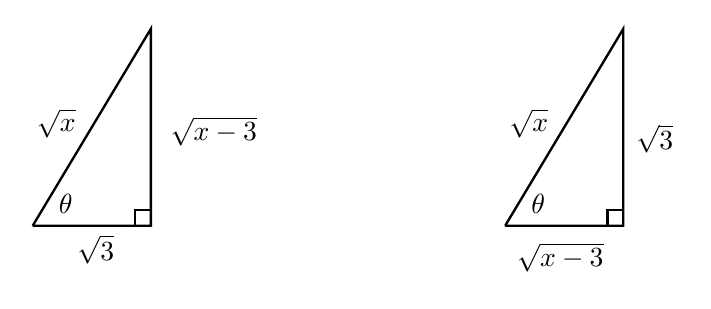
\begin{tikzpicture}
	\draw[line width=0.03cm] (0,0) -- (1.5,0) -- (1.5,2.5) -- (0,0);
	\draw[line width=0.03cm] (1.3,0) -- (1.3,0.2) -- (1.5,0.2);
	\node at (0.8,-0.3) {$\sqrt{3}$};
	\node at (2.3,1.2) {$\sqrt{x - 3}$};
	\node at (0.3,1.3) {$\sqrt{x}$};
	\node at (0.42,0.28) {$\theta$};
	
	\tikzset{shift={(6,0)}};

	\draw[line width=0.03cm] (0,0) -- (1.5,0) -- (1.5,2.5) -- (0,0);
	\draw[line width=0.03cm] (1.3,0) -- (1.3,0.2) -- (1.5,0.2);
	\node at (1.9,1.1) {$\sqrt{3}$};
	\node at (0.7,-0.4) {$\sqrt{x - 3}$};
	\node at (0.3,1.3) {$\sqrt{x}$};
	\node at (0.42,0.28) {$\theta$};
	\end{tikzpicture}
	\]
\itshape Alternatively, using the right triangle on the right, we have $\sin \theta= \tfrac{\sqrt{3}}{\sqrt{x}}$, so that $\sqrt{x}= \tfrac{\sqrt{3}}{\sin \theta}= \sqrt{3} \csc \theta$. So, $x= (\sqrt{x})^2= (\sqrt{3} \csc \theta)^2= 3 \csc^2 \theta$. But then $dx= 6 \csc \theta \cdot -\csc \theta \cot \theta \;d\theta= -6 \csc^2 \theta \cot \theta \;d\theta$. Observe that $\cot \theta= \frac{\sqrt{x - 3}}{\sqrt{3}}$, so that $\sqrt{x - 3}= \sqrt{3} \cot \theta$. But then\dots
	\[
	\int x \sqrt{x - 3} \;dx= \int 3 \csc^2 \theta (\sqrt{3} \cot \theta) \cdot -6 \csc^2 \theta \cot \theta \;d\theta= -\int 18 \sqrt{3} \csc^4 \theta \cot^2 \theta \;d\theta
	\]
We choose $u= \cot \theta$, so that $du= -\csc^2 \theta \;d\theta$. We know that $\sin^2 \theta + \cos^2 \theta= 1$, so that $1 + \cot^2 \theta= \csc^2 \theta$. But then\dots
	\[
	\hspace{-1.3cm} -\int 18 \sqrt{3} \csc^4 \theta \cot^2 \theta \;d\theta= 18 \sqrt{3} \int \cot^2 \theta \csc^2 \theta \cdot -\csc^2 \theta \;d\theta= 18 \sqrt{3} \int \cot^2 \theta (1 + \cot^2 \theta) \cdot -\csc^2 \theta \;d\theta
	\]
So, we have\dots
	\[
	\hspace{-1.8cm} 18 \sqrt{3} \int \cot^2 \theta (1 + \cot^2 \theta) \cdot -\csc^2 \theta \,d\theta= 18 \sqrt{3} \int u^2 (1 + u^2) \,du= 18\sqrt{3} \int \left( u^4 + u^2 \right) \,du= 18\sqrt{3} \left( \dfrac{u^5}{5} + \dfrac{u^3}{3} \right) + C
	\]
Using the fact that $u= \cot \theta$ and $\cot \theta= \tfrac{\sqrt{x - 3}}{\sqrt{3}}$, we have\dots
	\[
	\begin{aligned}
	18 \sqrt{3} \left( \dfrac{u^5}{5} + \dfrac{u^3}{3} \right) + C&= 50\sqrt{5} \left( \dfrac{\cot^5 \theta}{5} + \dfrac{\cot^3 \theta}{3} \right) + C \\
	&= \boxed{18 \sqrt{3} \left( \dfrac{1}{5}\, \left( \dfrac{\sqrt{x - 3}}{\sqrt{3}} \right)^5 + \dfrac{1}{3}\, \left( \dfrac{\sqrt{x - 3}}{\sqrt{3}} \right)^3 \right) + C} \\
	&= \dfrac{18\sqrt{3}}{15} \left( \dfrac{3(x - 3)^{5/2}}{3^{5/2}} + \dfrac{5(x - 3)^{3/2}}{3^{3/2}} \right) + C \\
	&= \dfrac{18 \sqrt{3}}{15 (3^{5/2})}\,(x - 3)^{3/2} \big( 3(x - 3) + 15 \big) + C \\
	&= \dfrac{2(3^2)(3^{1/2})}{5(3)(3^{5/2})}\,(x - 3)^{3/2} \left( 3x + 6 \right) + C \\
	&= \dfrac{2}{5(3)}\,(x - 3)^{3/2} \cdot 3 \left( x + 2 \right) + C \\
	&= \dfrac{2}{5}\,(x - 3)^{3/2} \left( x + 2 \right) + C 
	\end{aligned}
	\]
\setcounter{page}{7}
    }
}



% Question 7
\newpage
\question[10] Showing all your work and completely simplifying your result, compute the following:
	\[
	\int e^x \sin(5x) \;dx
	\] \par\vspace{0.1cm}

\vsol{\itshape Because this is of the form exponential function times sine or cosine, we recognize this as integration-by-parts---specifically a `looping' integral. Doing this the `long way', using LIATE, we choose $u= \sin(3x)$ and $dv= e^x$. We then have\dots
	{\footnotesize
	\[
	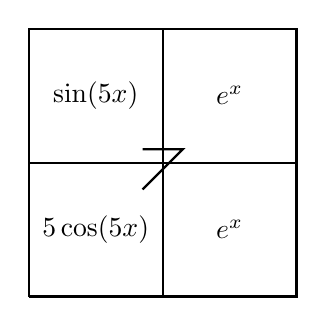
\begin{tikzpicture}[scale=0.85]
	\boxseven{\sin(5x)}{e^x}{5 \cos(5x)}{e^x}
	\end{tikzpicture}
	\]
	}
Therefore, we have\dots
	\[
	\int e^x \sin(5x) \;dx= e^x \sin(5x) - \int 5 e^x \cos(5x) \;dx
	\]
We now use LIATE again and choose $u= 5 \cos(5x)$ and $dv= e^x$. We then have\dots
	{\footnotesize
	\[
	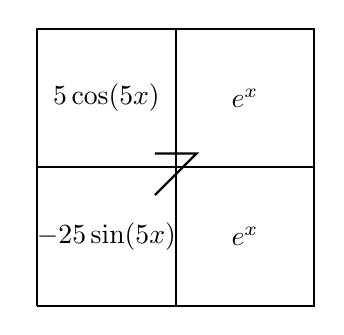
\begin{tikzpicture}[scale=0.88]
	\boxseven{ 5 \cos(5x)}{e^x}{-25 \sin(5x)}{e^x}
	\end{tikzpicture}
	\]
	}
So that\dots
	\[
	\begin{gathered}
	\hspace{-1.1cm} \int e^x \sin(5x) \;dx= e^x \sin(5x) - \int 5 e^x \cos(5x) \;dx \\[0.1cm]
	\int e^x \sin(5x) \;dx= e^x \sin(5x) - \left( 5e^x \cos(5x) - \int -25e^x \sin(5x) \;dx \right) \\[0.1cm]
	\int e^x \sin(5x) \;dx= e^x \sin(5x) - 5e^x \cos(3x) + \int -25e^x \sin(3x) \;dx \\[0.1cm]
	\int e^x \sin(5x) \;dx= e^x \sin(5x) - 5e^x \cos(3x) - 25 \int e^x \sin(3x) \;dx \\[0.1cm]
	26 \int e^x \sin(5x) \;dx= e^x \sin(5x) - 5e^x \cos(5x) \\[0.1cm]
	\int e^x \sin(5x) \;dx= \boxed{\dfrac{e^x \sin(5x) - 5e^x \cos(5x)}{26} + C} \\[0.1cm]
	\int e^x \sin(5x) \;dx= \dfrac{e^x}{26}\, \big( \sin(5x) - 5 \cos(5x) \big) + C
	\end{gathered}
	\]
}

\vsol{
\newpage
{
\thispagestyle{empty}
\itshape Alternatively, we can use tabular integration:
	\[
	\begin{array}{c @{\hspace*{1.3cm}} c} \toprule
	u & dv \\ \cmidrule(lr){1-2}
	\sin(5x) \tikzmark{Left 1} & \tikzmark{Right 1} e^x \\[0.5cm]
	5 \cos(5x) \tikzmark{Left 2} & \tikzmark{Right 2} e^x \\[0.3cm]
	-25 \sin(5x) \tikzmark{Left 3}  & \tikzmark{Right 3} e^x
	
	\DrawArrow{Left 1}{Right 2}{+}
	\DrawArrow{Left 2}{Right 3}{--}
	\DrawArrow{Left 3}{Right 3}{\!\!\!\!\!$\phantom{}_{\genfrac{}{}{0pt}{}{}{+}}$}
	\end{array}
	\] 
Therefore, we have\dots
	\[
	\begin{gathered}
	\int e^x \sin(3x) \;dx= e^x \sin(5x) - 5e^x \cos(5x) - 25 \int e^x \sin(5x) \;dx \\[0.1cm]
	26 \int e^x \sin(3x) \;dx= e^x \sin(5x) - 5e^x \cos(5x) \\[0.1cm]
	\int e^x \sin(3x) \;dx= \boxed{\dfrac{e^x \sin(5x) - 5e^x \cos(5x)}{26} + C} \\[0.1cm]
	\int e^x \sin(3x) \;dx= \dfrac{e^x}{26}\, \big( \sin(5x) - 5 \cos(5x) \big) + C
	\end{gathered}
	\]
\setcounter{page}{8}
   }
}



% Question 8
\newpage
\question[10] Showing all your work and completely simplifying your result, compute the following:
	\[
	\int \dfrac{3}{x^2 \sqrt{x^2 + 9}} \;dx
	\] \par\vspace{0.3cm}

\vsol{\itshape We know from the Pythagorean Theorem that $a^2 + b^2= c^2$. Taking $a^2= x^2$, i.e. $a= x$, and $b^2= 9$, i.e. $b= 3$, we have $c^2= a^2 + b^2= x^2 + 9$. This also shows that $c= \sqrt{x^2 + 9}$. There are two possible right triangles corresponding to these sides we could draw:
	\[
	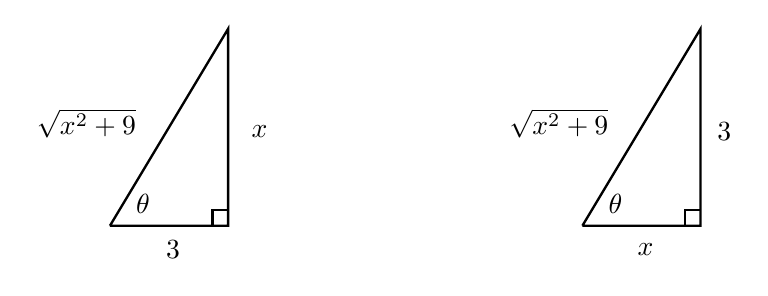
\begin{tikzpicture}
	\draw[line width=0.03cm] (0,0) -- (1.5,0) -- (1.5,2.5) -- (0,0);
	\draw[line width=0.03cm] (1.3,0) -- (1.3,0.2) -- (1.5,0.2);
	\node at (0.8,-0.3) {$3$};
	\node at (1.9,1.2) {$x$};
	\node at (-0.3,1.3) {$\sqrt{x^2 + 9}$};
	\node at (0.42,0.28) {$\theta$};
	
	\tikzset{shift={(6,0)}};

	\draw[line width=0.03cm] (0,0) -- (1.5,0) -- (1.5,2.5) -- (0,0);
	\draw[line width=0.03cm] (1.3,0) -- (1.3,0.2) -- (1.5,0.2);
	\node at (0.8,-0.3) {$x$};
	\node at (1.8,1.2) {$3$};
	\node at (-0.3,1.3) {$\sqrt{x^2 + 9}$};
	\node at (0.42,0.28) {$\theta$};
	\end{tikzpicture}
	\]
Using the right triangle on the left, we have $\tan \theta= \frac{x}{3}$, so that $x= 3 \tan \theta$. But then $dx= 3 \sec^2 \theta \;d\theta$. Because $x= 3 \tan \theta$, we know $x^2= 9 \tan^2 \theta$. Now observe that $\cos \theta= \frac{3}{\sqrt{x^2 + 9}}$. But then $\sqrt{x^2 + 9}= \frac{3}{\cos \theta}= 3 \sec \theta$. But then\dots
	\[
	\int \dfrac{3}{x^2 \sqrt{x^2 + 9}} \;dx= \int \dfrac{3}{9 \tan^2 \theta \cdot 3 \sec \theta} \cdot 3 \sec^2 \theta \;d\theta= \int \dfrac{\cancel{9} \sec^{\cancel{2}} \theta}{\cancel{27}^{\,3} \tan^2 \theta \cancel{\sec \theta}} \;d\theta= \dfrac{1}{3} \int \dfrac{\sec \theta}{\tan^2 \theta} \;d\theta
	\]
Using the fact that $\sec\theta= \frac{1}{\cos \theta}$ and $\tan \theta= \frac{\sin \theta}{\cos \theta}$, we have\dots
	\[
	\dfrac{1}{3} \int \dfrac{\sec \theta}{\tan^2 \theta} \;d\theta= \dfrac{1}{3} \int \dfrac{1/(\cos \theta)}{\left( \tfrac{\sin \theta}{\cos \theta} \right)^2} \;d\theta= \dfrac{1}{3} \int \dfrac{1}{\cos \theta} \cdot \dfrac{\cos^2 \theta}{\sin^2 \theta} \;d\theta= \dfrac{1}{3} \int \dfrac{1}{\cancel{\cos \theta}} \cdot \dfrac{\cos^{\cancel{2}} \theta}{\sin^2 \theta} \;d\theta= \dfrac{1}{3} \int \dfrac{\cos \theta}{\sin^2 \theta} \;d\theta
	\]
But then\dots
	\[
	\dfrac{1}{3} \int \dfrac{\cos \theta}{\sin^2 \theta} \;d\theta= \dfrac{1}{3} \int \dfrac{\cos \theta}{\sin \theta} \cdot \dfrac{1}{\sin \theta} \;d\theta= \dfrac{1}{3} \int \cot \theta \csc \theta \;d\theta= -\dfrac{1}{3} \int -\csc \theta \cot \theta \;d\theta= -\dfrac{\csc \theta}{3} + C
	\]
Alternatively, we could have chosen $u= \sin \theta$, so that $du= \cos \theta \;d\theta$. This would have given\dots
	\[
	\dfrac{1}{3} \int \dfrac{\cos \theta}{\sin^2 \theta} \;d\theta= \dfrac{1}{3} \int \dfrac{1}{\sin^2 \theta} \cdot \cos \theta \;d\theta= \dfrac{1}{3} \int \dfrac{1}{u^2} \;du= -\dfrac{1}{3u} + C= -\dfrac{1}{3 \sin \theta} + C= -\dfrac{\csc \theta}{3} + C
	\]
But from the right-triangle on the left, we know that $\csc \theta= \frac{\sqrt{x^2 + 9}}{x}$. Therefore, we have\dots
	\[
	\int \dfrac{3}{x^2 \sqrt{x^2 + 9}} \;dx= -\dfrac{\csc \theta}{3} + C= -\dfrac{1}{3} \cdot \frac{\sqrt{x^2 + 9}}{x} + C= -\frac{\sqrt{x^2 + 9}}{3x} + C
	\]
}

\vsol{
\newpage
{
\thispagestyle{empty}
	\[
	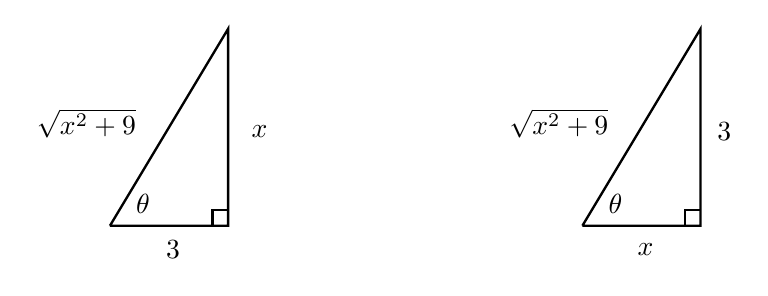
\begin{tikzpicture}
	\draw[line width=0.03cm] (0,0) -- (1.5,0) -- (1.5,2.5) -- (0,0);
	\draw[line width=0.03cm] (1.3,0) -- (1.3,0.2) -- (1.5,0.2);
	\node at (0.8,-0.3) {$3$};
	\node at (1.9,1.2) {$x$};
	\node at (-0.3,1.3) {$\sqrt{x^2 + 9}$};
	\node at (0.42,0.28) {$\theta$};
	
	\tikzset{shift={(6,0)}};

	\draw[line width=0.03cm] (0,0) -- (1.5,0) -- (1.5,2.5) -- (0,0);
	\draw[line width=0.03cm] (1.3,0) -- (1.3,0.2) -- (1.5,0.2);
	\node at (0.8,-0.3) {$x$};
	\node at (1.8,1.2) {$3$};
	\node at (-0.3,1.3) {$\sqrt{x^2 + 9}$};
	\node at (0.42,0.28) {$\theta$};
	\end{tikzpicture}
	\]
\itshape Alternatively, using the right triangle on the right, we have $\tan \theta= \frac{3}{x}$, so that $x= \frac{3}{\tan \theta}= 3 \cot \theta$. But then $dx= -3\csc^2 \theta \;d\theta$. Because $x= 3 \cot \theta$, we know $x^2= 3 \cot^2 \theta$. Now observe that $\sin \theta= \frac{3}{\sqrt{x^2 + 9}}$. But then $\sqrt{x^2 + 9}= \frac{3}{\sin \theta}= 3 \csc \theta$. But then\dots
	\[
	\int \dfrac{3}{x^2 \sqrt{x^2 + 9}} \;dx= \int \dfrac{3}{9 \cot^2 \theta \cdot 3 \csc \theta} \cdot -3\csc^2 \theta \;d\theta= \int \dfrac{\cancel{-9}^{\,-1} \csc^{\cancel{2}} \theta}{\cancel{27}^{\,2} \cot^2 \theta \cancel{\csc \theta}} \;d\theta= -\dfrac{1}{3} \int \dfrac{\csc \theta}{\cot^2 \theta} \;d\theta
	\]
Using the fact that $\csc\theta= \frac{1}{\sin \theta}$ and $\cot \theta= \frac{\cos \theta}{\sin \theta}$, we have\dots
	\[
	\hspace{-1.3cm} -\dfrac{1}{3} \int \dfrac{\csc \theta}{\cot^2 \theta} \;d\theta= -\dfrac{1}{3} \int \dfrac{1/(\sin \theta)}{\left( \tfrac{\cos \theta}{\sin \theta} \right)^2} \;d\theta= -\dfrac{1}{3} \int \dfrac{1}{\sin \theta} \cdot \dfrac{\sin^2 \theta}{\cos^2 \theta} \;d\theta= -\dfrac{1}{3} \int \dfrac{1}{\cancel{\sin \theta}} \cdot \dfrac{\sin^{\cancel{2}} \theta}{\cos^2 \theta} \;d\theta= -\dfrac{1}{3} \int \dfrac{\sin \theta}{\cos^2 \theta} \;d\theta
	\]
But then\dots
	\[
	-\dfrac{1}{3} \int \dfrac{\sin \theta}{\cos^2 \theta} \;d\theta= -\dfrac{1}{3} \int \dfrac{\sin \theta}{\cos \theta} \cdot \dfrac{1}{\cos \theta} \;d\theta= -\dfrac{1}{3} \int \tan \theta \sec \theta \;d\theta= -\dfrac{\sec \theta}{3} + C
	\]
Alternatively, we could have chosen $u= \cos \theta$, so that $du= -\sin \theta \;d\theta$. This would have given\dots
	\[
	-\dfrac{1}{3} \int \dfrac{\sin \theta}{\cos^2 \theta} \;d\theta= \dfrac{1}{3} \int \dfrac{1}{\cos^2 \theta} \cdot -\sin \theta \;d\theta= \dfrac{1}{3} \int \dfrac{1}{u^2} \;du= -\dfrac{1}{3u} + C= -\dfrac{1}{3 \cos \theta} + C= -\dfrac{\sec \theta}{3} + C
	\]
But from the right-triangle on the right, we know that $\sec \theta= \frac{\sqrt{x^2 + 4}}{x}$. Therefore, we have\dots
	\[
	\int \dfrac{3}{x^2 \sqrt{x^2 + 9}} \;dx= -\dfrac{\sec \theta}{3} + C= -\dfrac{1}{3} \cdot \frac{\sqrt{x^2 + 9}}{x} + C= -\frac{\sqrt{x^2 + 9}}{3x} + C
	\]

\setcounter{page}{9}
   }
}



% Question 9
\newpage
\question[10] Showing all your work and completely simplifying your result, compute the following:
	\[
	\int \dfrac{x^5}{x^{12} + 1} \;dx
	\] \par\vspace{0.3cm}

\vsol{\itshape We will make the $u$-substitution $u= x^6$, so that $du= 6x^5 \;dx$. But then\dots
	\[
	\begin{aligned}
	\int \dfrac{x^5}{x^{12} + 1} \;dx&= \int \dfrac{x^5}{(x^6)^2 + 1} \;dx \\[0.3cm]
	&= \dfrac{1}{6} \int \dfrac{6x^5}{(x^6)^2 + 1} \;dx \\[0.3cm] 
	&= \dfrac{1}{6} \int \dfrac{1}{u^2 + 1} \;du \\[0.3cm]
	&= \dfrac{1}{6}\, \arctan u + C \\[0.3cm]
	&= \boxed{\dfrac{\arctan(x^6)}{6} + C}
	\end{aligned}
	\]
}

\end{questions}
\end{document}